\documentclass[en]{sdqbeamer} 

%Preamble
\usepackage{amssymb}
\usepackage{amsmath}
\usepackage[export]{adjustbox}
\usepackage{pgf-pie}
\usepackage[citestyle=numeric, bibstyle=numeric, backend=biber]{biblatex}
\addbibresource{../latex/References.bib}
\bibhang1em
\setbeamertemplate{bibliography item}{\insertbiblabel}

\newenvironment{rcases}
{\left.\begin{aligned}}
	{\end{aligned}\right\rbrace}

%Title
\titleimage{banner_2020_kit}
\groupname{Research group for heterogeneous and parallel computing }
\title[Hardware Accelerators for Neural Networks]{A Survey on Hardware Accelerators for Neural Networks}
\author[Pierre Brosemer]{Pierre Brosemer}
\date[23.\,03.\,2020]{23. March 2020}

\begin{document}
	
	\KITtitleframe
	
	\begin{frame}{Table of contents}
		\tableofcontents
	\end{frame}
	
	\section{Fundamentals neural networks}
	\begin{frame}
		\begin{figure}
			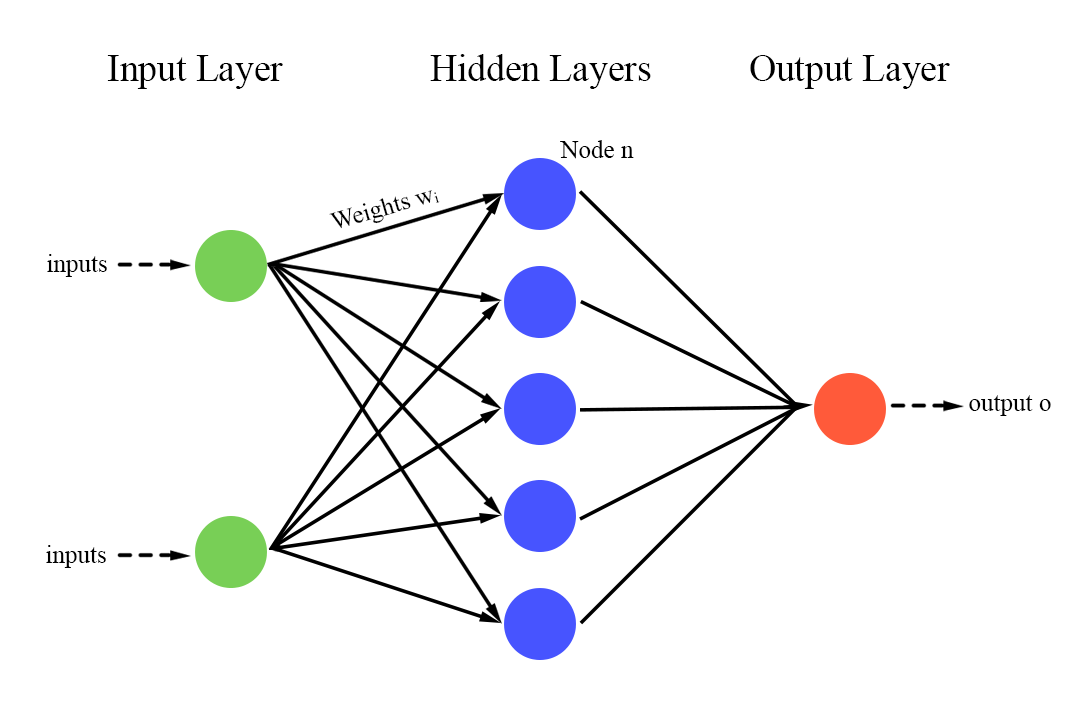
\includegraphics[width= 0.6\paperwidth]{pictures/neuralnetwork.png}
		\end{figure}
		\centering
		A typical representation of a neural network.
	\end{frame}
	
	\begin{frame}
		\begin{figure}
			\centering
			\begin{minipage}{0.45\paperwidth}
				\centering
				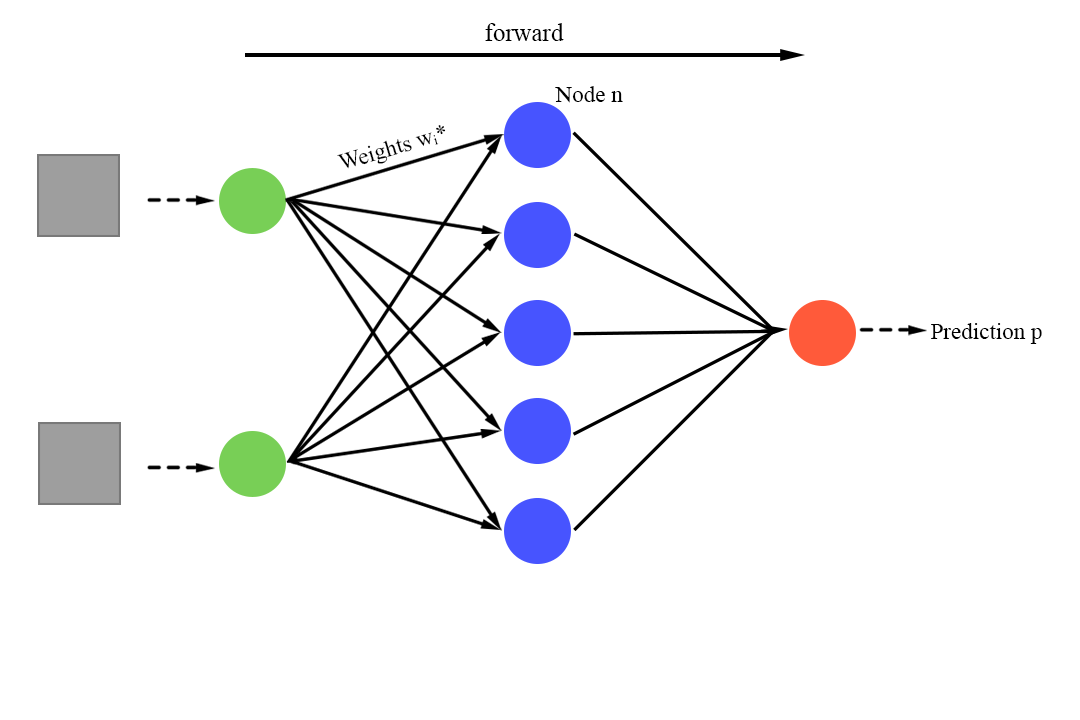
\includegraphics[width=0.45\paperwidth]{pictures/inference.png}
				\caption{Inference phase for a neural network.}
			\end{minipage}\vrule{}
			\begin{minipage}{0.45\paperwidth}
				\centering
				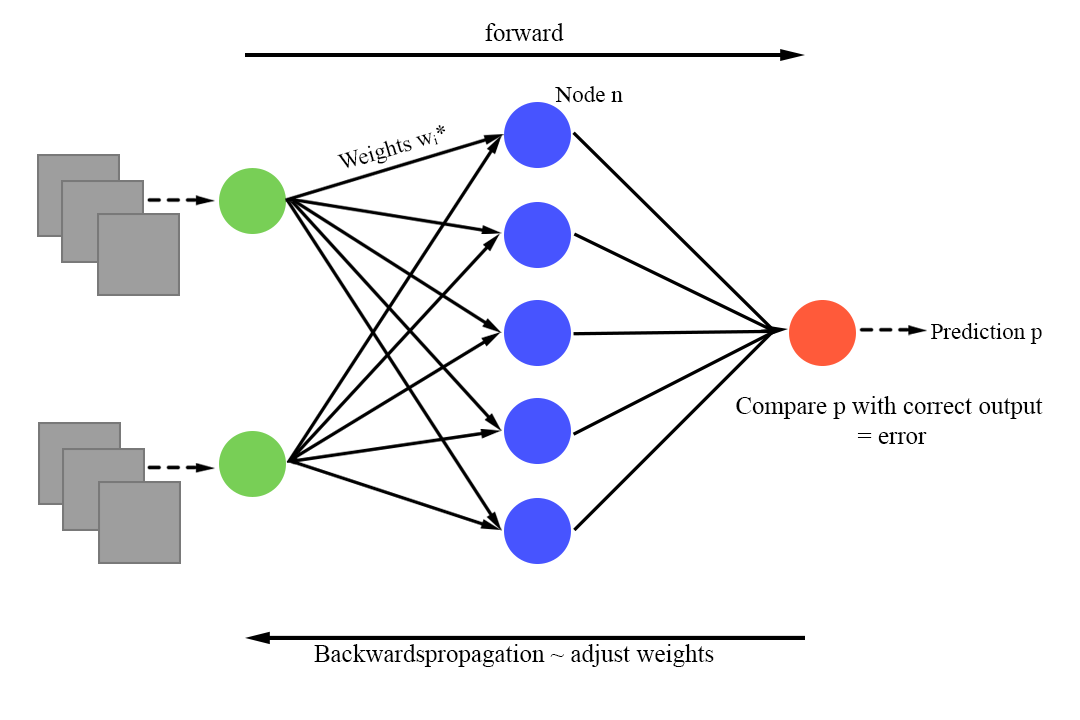
\includegraphics[width=0.45\paperwidth]{pictures/training.png}
				\caption{Training phase for a neural network.}
			\end{minipage}
		\end{figure}
		$\rightsquigarrow$ vast amount of computational power
	\end{frame}
	
	\section{Different types of hardware}
	\begin{frame}{Categorization}
		Four main types:
		\\
		\[
		\begin{rcases}
			\text{Central Processing Unit (CPU) } \\
			\text{Graphics Processing Unit (GPU) } 
		\end{rcases} \text{temporal architecture}
		\]
		\\
		\quad
		\\
		\[
		\begin{rcases}
			\text{Field-Programmable Gate Array (FPGA) } \\
			\text{Application-Specific Integrated Circuit (ASIC) }
		\end{rcases} \text{spatial architecture}
		\]
	\end{frame}
	
	\subsection{CPU}
	\begin{frame}{Central Processing Unit}
		Properties of a CPU:
		\begin{itemize}
			\item good at executing serial instructions in parallel
			\item small amount of cores
			\item fetches instructions and execute
		\end{itemize}
		$\rightsquigarrow$ Bad parallelization for the same instruction.\\ $\rightsquigarrow$ Slow training and inference phases. \cite{capra2020updated}
	\end{frame}
	
	\subsection{GPU}
	\begin{frame}{Graphics Processing Unit}
		\begin{minipage}[b]{0.45\paperwidth}
			Graphics Processing Unit
			\begin{itemize}
				\item specifications align with graphics rendering
				\item hundreds of cores with individual caches
				\item good parallelization of matrix multiplication
			\end{itemize}
		\end{minipage}
		\begin{minipage}{0.45\paperwidth}
			\begin{figure}
				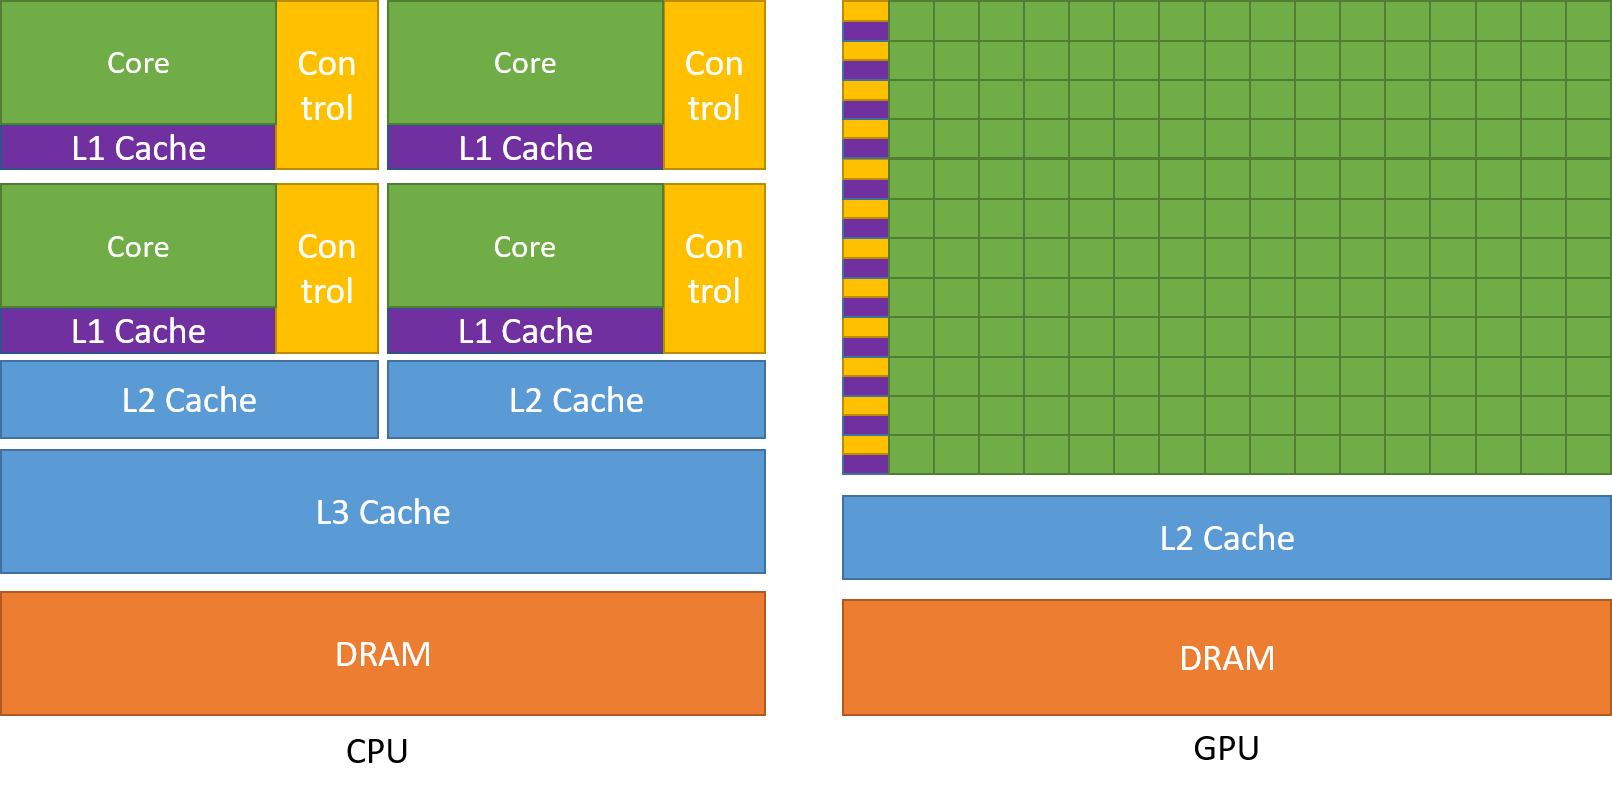
\includegraphics[width= 0.47\paperwidth, right]{pictures/intel_comparison.png}
				\caption{Layout differences between CPU and GPU \cite{intelpic_comparison}}
			\end{figure}
		\end{minipage}
	\end{frame}
	
	\begin{frame}{Acceleration by GPUs}
		Properties of GPUs for working with neural networks\cite{nvidiav100}:
		\begin{itemize}
			\item achieve fast matrix multiplications
			\item make use of sparsity in matrices
			\item mostly used for training
			\item high memory bandwidth
		\end{itemize}
	\end{frame}
	
	\subsection{FPGA}
	\begin{frame}{Field-Programmable Gate Array}
		General Properties:
		\begin{itemize}
			\item integrated circuit
			\item reprogramming with Hardware Description Language (HDL)
			\item limited flexibility compared to GPUs
			\item high compile times
		\end{itemize}
	\end{frame}
	
	\begin{frame}{Example speedup for a FPGA}
		Accelerating operation for recurrent neural networks \cite{nurvitadhi2016accelerating}:
		\begin{itemize}
			\item matrix divided into column blocks
			\item multiple FMA units
			\item each FMA unit responsible for one row in column block
			\item multiply rows to input vector
		\end{itemize}
	\end{frame}
	
	\begin{frame}
		\begin{figure}
			\centering
			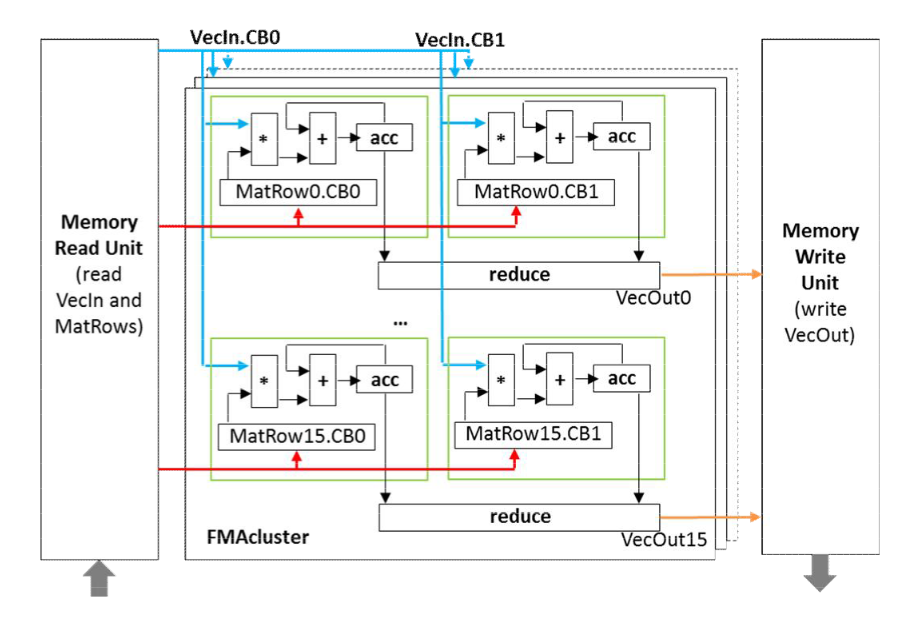
\includegraphics[width= 0.55\paperwidth]{pictures/fpga_operations.png}
			\caption{A simplified depiction showing the layout and dataflows of the previously mentioned FPGA \cite{nurvitadhi2016accelerating}}
		\end{figure}
	\end{frame}
	
	%Maybe Microsoft if enough Time
	
	\subsection{ASIC}
	\begin{frame}{Application-Specific Integrated Circuit}
		General Properties:
		\begin{itemize}
			\item integrated circuit
			\item can't be reprogrammed after production
			\item time-consuming and complicated process of design
			\item more energy-efficient than FPGAs
		\end{itemize}
	\end{frame}
	
	\begin{frame}{Tensor Processing Unit}
		Hardware was specifically built for inference phase \cite{jouppi2017datacenter}.\\
		Main components include:
		\begin{itemize}
			\item Matrix Multiply Unit (MMU)
			\item Unified Buffer
			\item Accumulators
		\end{itemize}
		Features:
		\begin{itemize}
			\item FIFO for weights
			\item systolic array for faster access
			\item 4-stage parallelism
		\end{itemize}
	\end{frame}
	
	\begin{frame}
		\begin{figure}
			\centering
			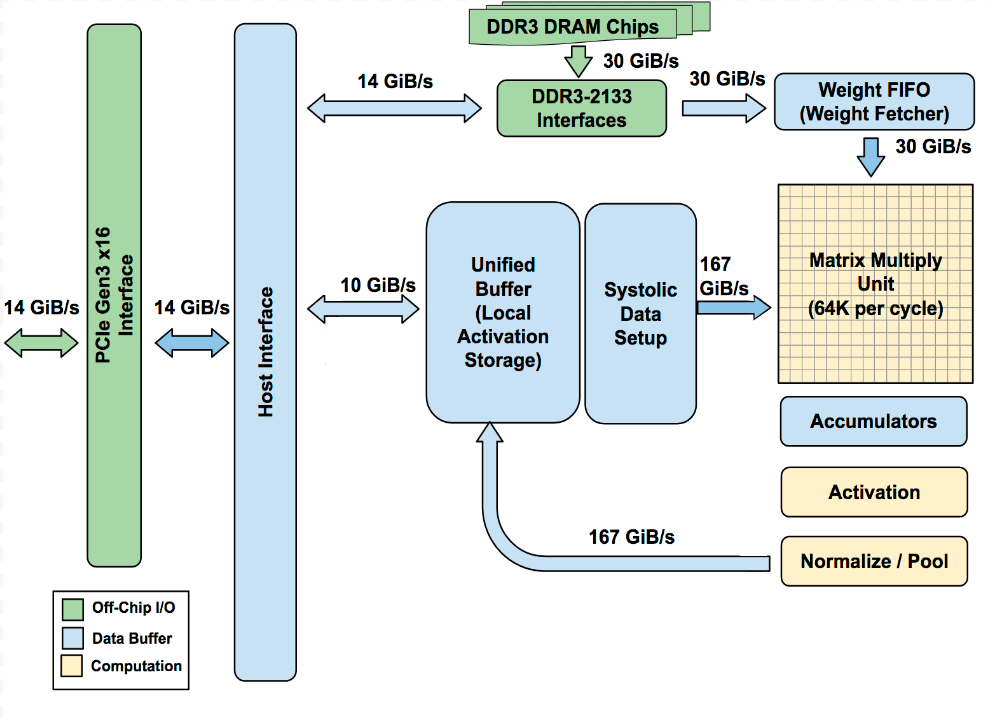
\includegraphics[width= 0.5\paperwidth]{pictures/tpu_floorplan.png}
			\caption{A simplified block diagram of the first version TPU. The left side represents the host (CPU). The host sends instructions to the TPU and receives a data back \cite{jouppi2017datacenter}.}
		\end{figure}
	\end{frame}
	
	% other TPU versions
	
	\section{Comparison}
	
	\begin{frame}{Metrics}
		Main metrics:
		\begin{itemize}
			\item performance: GOP/s billions of operations per second
			\item efficiency
			\item memory transfer rate
		\end{itemize}
		$\rightsquigarrow$ metrics hard to measure, mostly measured on target application
	\end{frame}
	
	\begin{frame}{MLPerf}
		Claims to be the industry standard for performance measuring for neural networks \cite{mattson2020mlperf}:
		\begin{itemize}
			\item founded by both members of science and industry
			\item fixed software configurations for testing the hardware accelerators
		\end{itemize}	
	\end{frame}
	
	\begin{frame}
		\begin{figure}
			\centering
			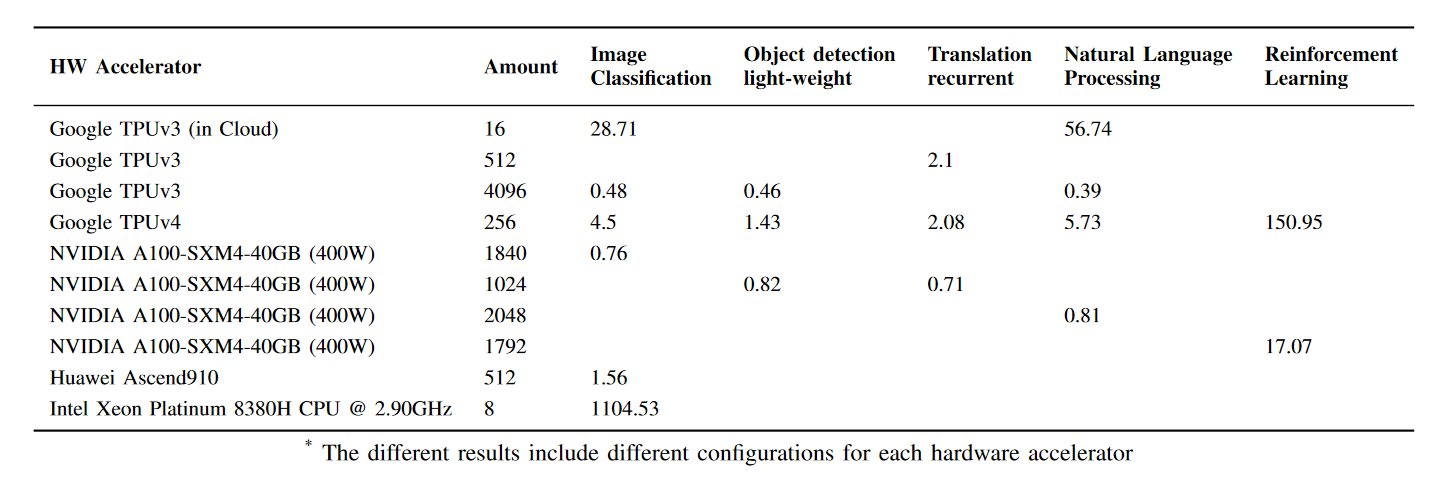
\includegraphics[width= 0.95\paperwidth]{pictures/table.png}
			\caption{A Table showing some results from the training in MLPerf v0.7 in the category Regular, Closed Division Times \cite{mlperfresults}.}
		\end{figure}
	\end{frame}
	
	\begin{frame}{Literature Review}
		\begin{minipage}[b]{0.45\paperwidth}
			Published literature for hardware accelerators:
			\begin{itemize}
				\item most commonly used accelerator FPGA
				\item $\rightsquigarrow$ good for prototyping 
				\item easy usage favours GPUs
			\end{itemize}
		\end{minipage}
		\begin{minipage}{0.45\paperwidth}
			\begin{figure}
				\centering
				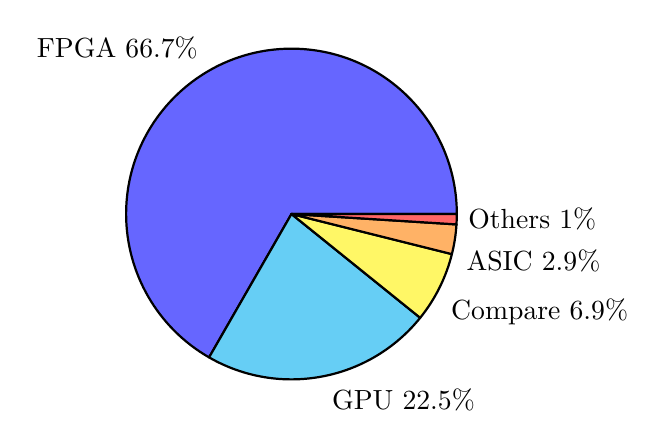
\begin{tikzpicture}[scale=0.7]
					\pie[hide number]{66.7/FPGA 66.7\%, 22.5/GPU 22.5\%, 6.9/Compare 6.9\%, 2.9/ASIC 2.9\%, 1/Others 1\%}
				\end{tikzpicture}
				\caption{The results percentages of the different hardware accelerators found in scientific papers \cite{talib2020systematic}.}
				\label{fig:piech}
			\end{figure}
		\end{minipage}
	\end{frame}

	\begin{frame}{General Comparison}
		Other things to note:
		\begin{itemize}
			\item GPUs are "workhorses" for traning neural networks \cite{capra2020updated}
			\item FPGAs more energy efficient \cite{blott2019qutibench}. Factor of up to 10x better \cite{ovtcharov2015accelerating}
		\end{itemize}
	\end{frame}

	\section{Hardware Accelerators in Edge Devices}
	\begin{frame}{Application in Edge Devices}
		Play a key role in bringing the services of neural networks to the application. \\
		Requirements \cite{wang2020convergence}:
		\begin{itemize}
			\item fast response times
			\item high reliability (loss of connection)
			\item limited energy and computation
		\end{itemize}
	\end{frame}

	\begin{frame}{Implementation}
		\begin{minipage}[b]{0.45\paperwidth}
			Optimizations include:
			\begin{itemize}
				\item optimize performance \cite{szegedy2015going} 
				\item reduce search space \cite{zhang2018ffs}
			\end{itemize}
		\end{minipage}
		\begin{minipage}{0.45\paperwidth}
			\begin{figure}
				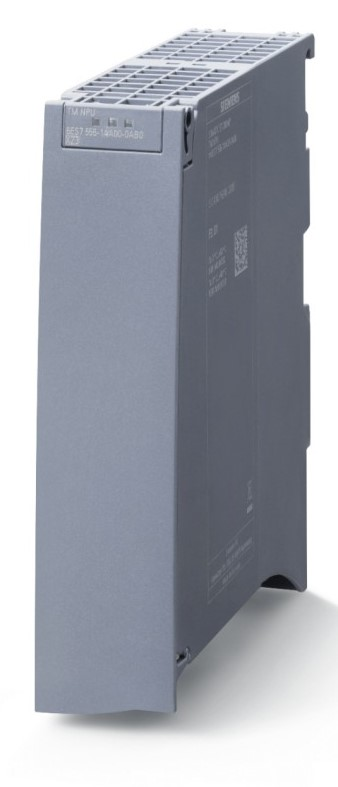
\includegraphics[width= 0.47\paperwidth, right]{pictures/siemens_npu.png}
				\caption{Module S7-1500 TM NPU (Neural Processing Unit) \cite{siemensnpu_pic}}
			\end{figure}
		\end{minipage}
	\end{frame}
	
	\begin{frame}{Conclusion}
		Main takeaways:
		\begin{itemize}
			\item important role in bringing neural networks to application
			\item choosing accelerators application-specific
			\item ongoing research
		\end{itemize}
	\end{frame}

	\appendix
	\beginbackup
	
	\begin{frame}{References}
		\printbibliography
	\end{frame}
	
\end{document}